\documentclass{exam}
\usepackage{tikz}
\usepackage{amssymb}
\usepackage{amsmath}
\title{CS113/DISCRETE MATHEMATICS-SPRING 2024}
\author{Worksheet 26}
\date{Topic: Euler Path And Circuits }
\begin{document}
\maketitle
\vspace{5mm}
\begin{center}
\fbox{\fbox{\parbox{5.5in}{\centering Now, that we have covered Graph connectivity in last class, we shall move on to different types of circuits and paths.Today, we will explore Euler paths which allow us to navigate from one vertex to another, covering every edge exactly once as well as Euler circuits which take us on a journey where we start and end at the same vertex, visiting each edge only once. Happy Learning!}}}
\end{center}
\vspace{5mm}

\makebox[0.75\textwidth]{Student's Name and ID:\enspace\hrulefill} 

\vspace{5mm}
\makebox[0.75\textwidth]{Instructor’s name:\enspace\hrulefill}

\vspace{10mm}




\begin{questions}

\question
For the given parts, determine whether the given graph has an
Euler circuit. Construct such a circuit when one exists. If
no Euler circuit exists, determine whether the graph has an
Euler path and construct such a path if one exists.
\begin{parts}
\part
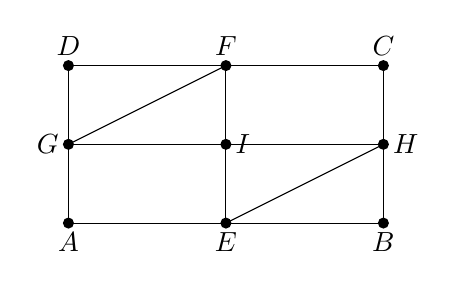
\begin{tikzpicture}
  % Define the coordinates for the rectangle vertices
  \coordinate[label=below:$A$] (A) at (0,0);
  \coordinate[label=below:$B$] (B) at (4,0);
  \coordinate[label=above:$C$] (C) at (4,2);
  \coordinate[label=above:$D$] (D) at (0,2);
  \coordinate[label=below:$E$] (E) at (2,0);
  \coordinate[label=above:$F$] (F) at (2,2);
  \coordinate[label=left:$G$] (G) at (0,1);
  \coordinate[label=right:$H$] (H) at (4,1);
  \coordinate[label=right:$I$] (I) at (2,1);

  % Draw the rectangle
  \draw (A) -- (B) -- (C) -- (D) -- cycle;
  \draw (F)--(I)--(E);
  \draw (G)--(I)--(H);
  \draw (G)--(F);
  \draw (E)--(H);
  \foreach \vertex in {A, B, C, D,E,F,G,H,I}
    \fill (\vertex) circle (2pt);
  
\end{tikzpicture}
\newpage

\part 
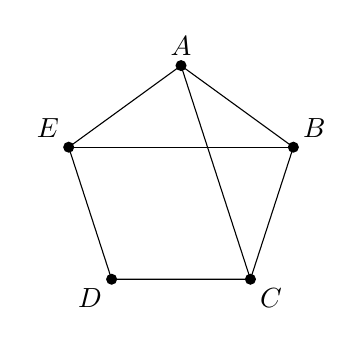
\begin{tikzpicture}
  % Define the coordinates for the pentagon vertices
  \coordinate[label=above:$A$] (A) at (90:1.5);
  \coordinate[label=above right:$B$] (B) at (18:1.5);
  \coordinate[label=below right:$C$] (C) at (-54:1.5);
  \coordinate[label=below left:$D$] (D) at (-126:1.5);
  \coordinate[label=above left:$E$] (E) at (162:1.5);

  % Draw the pentagon
  \draw (A) -- (B) -- (C) -- (D) -- (E) -- cycle;
  \draw (B)--(E);
  \draw (A)--(C);

  % Add points at the vertices (optional)
  \foreach \vertex in {A, B, C, D, E}
    \fill (\vertex) circle (2pt);
\end{tikzpicture}
\newpage

\part
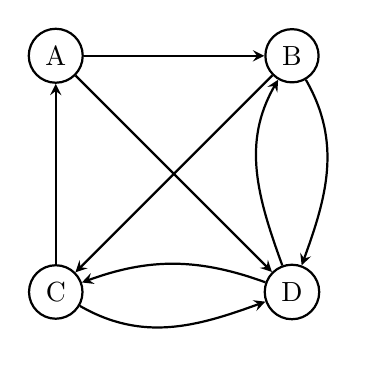
\begin{tikzpicture}[->,>=stealth,auto,node distance=2.5cm,thick]
  % Define the vertices
  \node[circle,draw] (C) at (0,0) {C};
  \node[circle,draw] (D) at (3,0) {D};
  \node[circle,draw] (B) at (3,3) {B};
  \node[circle,draw] (A) at (0,3) {A};

  % Add the directed edges

  \draw (B) edge[out=-60, in=70] (D);
  \draw (D) edge[out=160, in=20] (C);
  \draw (D) edge[out=110, in=240] (B);
  \draw (C) edge[out=330, in=200] (D);
  \draw (A)->(B);
  \draw (C)->(A);
  \draw (A)->(D);
  \draw (B)->(C);
  
\end{tikzpicture}
\newpage

\part
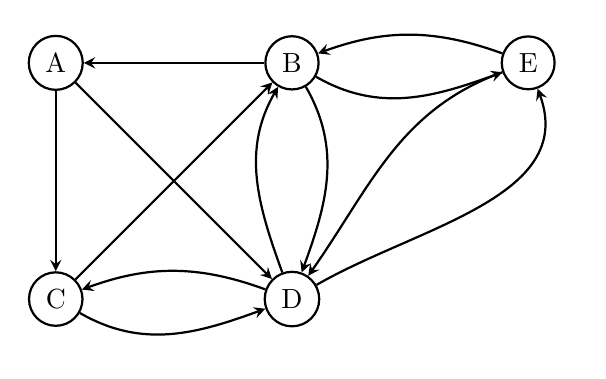
\begin{tikzpicture}[->,>=stealth,auto,node distance=2.5cm,thick]
  % Define the vertices
  \node[circle,draw] (C) at (0,0) {C};
  \node[circle,draw] (D) at (3,0) {D};
  \node[circle,draw] (B) at (3,3) {B};
  \node[circle,draw] (A) at (0,3) {A};
  \node[circle,draw] (E) at (6,3) {E};

  % Add the directed edges

  \draw (B) edge[out=-60, in=70] (D);
  \draw (D) edge[out=160, in=20] (C);
  \draw (D) edge[out=110, in=240] (B);
  \draw (C) edge[out=330, in=200] (D);
  \draw (E) edge[out=160, in=20] (B);
  \draw (B) edge[out=330, in=200] (E);
  \draw (E) edge[out=200, in=55] (D);
  \draw (D) edge[out=30, in=290] (E);
  \draw (B)->(A);
  \draw (A)->(C);
  \draw (A)->(D);
  \draw (C)->(B);
  
\end{tikzpicture}
\newpage

\end{parts}
\end{questions}
\end{document}




